\chapter{Proposed Methodology}
\label{ch:method}

\section{Dataset Description}
\label{sec:dataset}

The project uses the Jinan and Hangzhou datasets that were released with CoLight
\citep{wei2019colight} in the input format of the CityFlow simulator \citep{zhang2019cityflow}.
Each city comes with one road network file and three flow files. A flow file covers one hour
of traffic and gives, for every vehicle, the second at which it enters (0--3599) and its route
as an ordered list of roads. The release says the trips were reconstructed from roadside camera
records. In this project the data is the \emph{environment}, since the agents learn from
transitions that come out of simulating the training flow. \Cref{tab:data} lists the files.

\begin{table}[t]
\centering\small
\caption[Datasets and split]{Datasets and split. Whole flow files are assigned to splits; Hangzhou is never
simulated before the final evaluation.}
\label{tab:data}
\begin{tabular}{llrrl}
\toprule
City, network & Flow file & Vehicles & Roads per route & Role \\
\midrule
Jinan, $3\times4$ grid, & \texttt{jinan\_real} & 6295 & 2--17 (mean 4.4) & train: fits the weights \\
12 signalised intersections, & \texttt{jinan\_real\_2000} & 4365 & 2--19 (mean 4.4) & validation: all selection \\
roads of 400 and 800\,m & \texttt{jinan\_real\_2500} & 5494 & 2--17 (mean 4.4) & test: run once \\
\midrule
Hangzhou, $4\times4$ grid, & \texttt{hangzhou\_real} & 2983 & 2--16 (mean 4.7) & held-out city (flow A) \\
16 signalised intersections, & \texttt{hangzhou\_real\_5734} & 6538 & 2--16 (mean 4.7) & held-out city (flow B) \\
roads of 600 and 800\,m & \texttt{hangzhou\_real\_5816} & 6984 & 2--17 (mean 4.6) & held-out city (flow C) \\
\bottomrule
\end{tabular}
\end{table}

All roads have three lanes (left, through, right) and a 40\,km/h speed limit. A signalised
intersection has four approaches with twelve movements between them, eight green phases and a
5\,s transition phase. There is a single vehicle class, so all vehicles share one parameter set.

\textbf{Licence and privacy.} The source repository has no licence file. The data is treated
as publicly released research data, used for coursework only and not redistributed, and
each file is pinned by its SHA-256 hash. The files hold no vehicle identifier, number plate,
date or personal attribute.

\textbf{Audit.} A scripted audit ran 17 checks over the 32\,659 vehicle records (missing
fields, wrong types, duplicates, start times outside the hour, unknown roads, disconnected
routes) and 12 checks over the two road networks. None of them found a defect, and the data is
used as released. Three oddities are kept and reported. Between 1 and 2\,\% of trips end inside
the network, 3--4\,\% of routes cross the same intersection twice, and the Jinan training flow
has a five-minute stretch of low demand.

\section{Data Preprocessing}
\label{sec:prep}

\textbf{Split and leakage control.} Whole files go to the splits before any other step
(\cref{tab:data}); nothing is resampled or shared between splits, and Hangzhou is held out as a
whole city. Flow files can only be loaded through one function, which checks the hash and
refuses the test and held-out files unless a final-evaluation flag is set. The training flow
fits the network weights, and the validation flow is used to pick the checkpoint, the
hyperparameters and the gate threshold. The test and held-out flows were run once, after a hash
manifest had locked the models.

\textbf{Features.} Each intersection $i$ observes 44 values,
\begin{equation}
s_i=\big[\,q_i \,\|\, x_i \,\|\, \pi_i \,\|\, \mathrm{onehot}(\phi_i)\,\big],\qquad
q_{i,l}=\min\!\Big(1,\frac{w_l}{c_l}\Big),\quad
x_{i,l}=\min\!\Big(1,\frac{n_l}{c_l}\Big),\quad
\pi_{i,m}=\bar x_{\mathrm{in}(m)}-\bar x_{\mathrm{out}(m)},
\label{eq:state}
\end{equation}
where $w_l$ and $n_l$ count the waiting and the total vehicles on incoming lane $l$ (12
lanes), $\pi_{i,m}$ is the pressure of movement $m$ (12 movements), $\phi_i$ is the current
green phase (8 values) and $c_l=\lfloor \mathrm{length}_l/7.5\,\mathrm{m}\rfloor$ is the lane
capacity. Capacity follows from the length of the road, so \emph{no statistic is fitted on
data}. Nothing can leak from the validation or test flows this way, and the scaling carries
over to Hangzhou as it is. Lanes are always stored in the same order (approaches E, N, W, S,
each with left, through and right lanes), which lets one network serve every intersection.

\section{Exploratory Data Analysis (EDA)}
\label{sec:eda}

The EDA simulated the training flow alone under three rule controllers (Fixed-Time,
Max-Pressure and random phases). What it showed fixed the design choices below, all before any
learning agent was trained.
\begin{itemize}
\item \emph{Demand} moves in five-minute blocks between roughly 3000 and 8160 vehicles per
hour, so a single episode passes through several demand levels. The load is also uneven, with
1477 to 2058 vehicles per hour at different intersections.
\item \emph{No lane} goes above 96\,\% of its capacity, so scaling by capacity
(\cref{eq:state}) keeps the inputs in range.
\item \emph{No steady state}: waiting vehicles pile up through the hour under every
controller, and 13--21\,\% of trips are unfinished at the end. Since the results depend on
how long the episode runs, it is fixed at 3600\,s, and throughput and maximum wait are
reported alongside the mean travel time.
\item \emph{Reward proxy}: the queue at an intersection and its absolute pressure correlate at
0.65--0.82. Pressure drops to about zero when the incoming and outgoing lanes are both full,
though, so it serves as the reward (\cref{eq:reward}) and is never used to evaluate.
\item \emph{Decision interval} (\cref{fig:eda}): with $\dt=5$, 10, 15 and 20\,s,
Max-Pressure reaches an average travel time of 451, 375, 344 and 347\,s. Short intervals waste
green time on the 5\,s transitions, and $\dt=15$\,s was fixed for every controller.
\item \emph{Determinism}: a rule controller gives the same result for every seed, so it has
no confidence interval.
\end{itemize}

\begin{figure}[t]
\centering
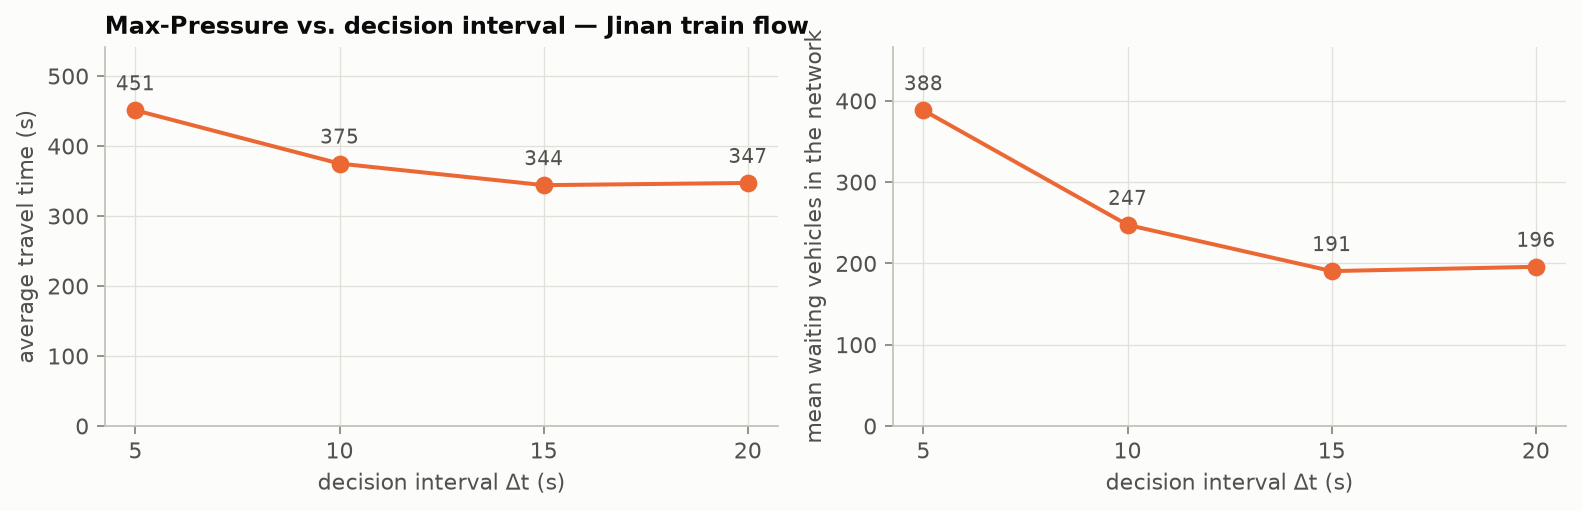
\includegraphics[width=0.62\textwidth]{10_decision_interval.png}
\caption[EDA: Max-Pressure against the decision interval (training flow)]{EDA on the Jinan training flow: Max-Pressure with a decision every $\dt$ seconds.
Average travel time (left) and mean number of waiting vehicles (right) are lowest at
$\dt=15$\,s, the value frozen in the evaluation protocol.}
\label{fig:eda}
\end{figure}

\section{Proposed Model Architecture}
\label{sec:arch}

\Cref{fig:arch} shows the whole system. One network serves all intersections. It encodes
an intersection's observation along with those of its neighbours and scores each phase with
$K$ heads. When the heads disagree too much, the Max-Pressure phase is applied in place of the
learned one.

\begin{figure}[t]
\centering
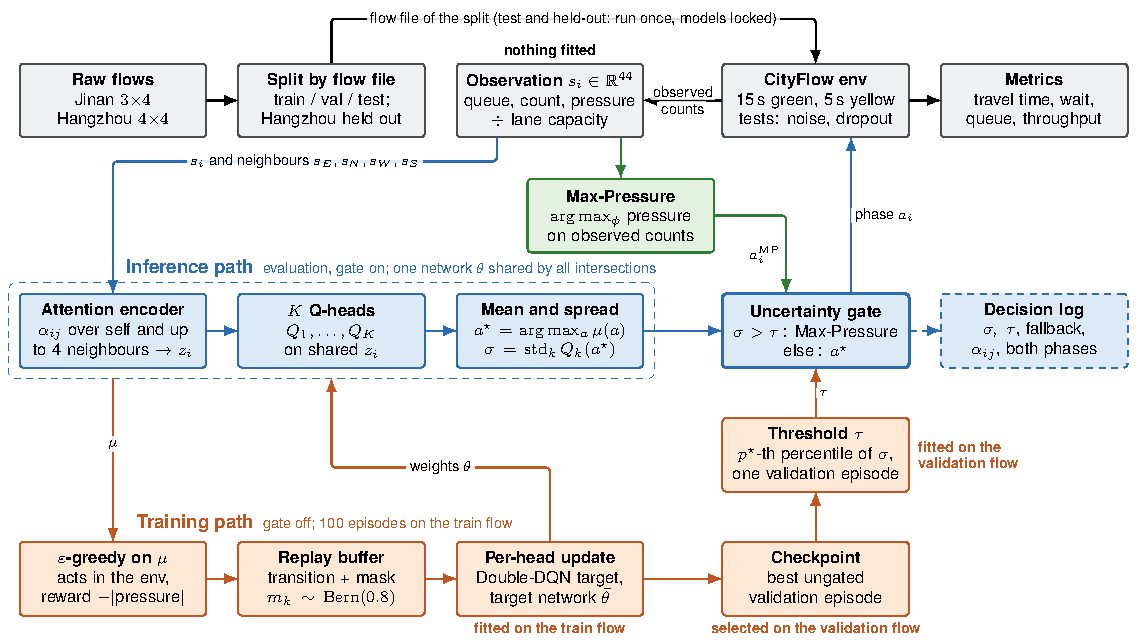
\includegraphics[width=\textwidth]{architecture.pdf}
\caption[\ugmarl{} architecture: data, inference path and training path]{\ugmarl{} architecture in data-flow order. Grey: data and environment. Blue:
inference path with the uncertainty gate. Green: the Max-Pressure fallback. Orange:
training path. Tags mark what is fitted on the training flow and what is fitted or
selected on the validation flow; the observation scaling fits nothing.}
\label{fig:arch}
\end{figure}

\subsection{Decision process}
Every intersection runs on its own clock. When it is ready, it picks the next green phase
$a_i\in\{1,\dots,8\}$ and holds it for $\dt=15$\,s, with 5\,s of transition first whenever the
phase changes. One decision interval therefore lasts $d\in\{15,20\}$\,s, intersections decide
at different moments, and each one faces a semi-Markov decision process. The reward is minus
the absolute pressure at the end of the interval,
\begin{equation}
r_i=-\lvert P_i\rvert,\qquad P_i=\sum_{l\in \mathrm{in}(i)} n_l-\sum_{l\in \mathrm{out}(i)} n_l ,
\label{eq:reward}
\end{equation}
which is the quantity Max-Pressure drives down \citep{varaiya2013max,wei2019presslight}.
The learned policy and its fallback therefore work towards the same goal.

\subsection{Learning target}
The three learned agents (DQN, IDQN and \ugmarl{}) are trained with the Double Q-learning
target, a target network $\bar\theta$, uniform replay and the Huber loss. For a transition
$(s,a,r,s',d)$,
\begin{equation}
y = c\,r+\gamma^{\,d/\dt}\,Q_{\bar\theta}\big(s',\argmax_{a'}Q_\theta(s',a')\big),\qquad
\mathcal L(\theta)=\mathrm{Huber}\big(Q_\theta(s,a)-y\big),
\label{eq:target}
\end{equation}
where the reward scale is fixed at $c=0.01$. Because intervals have different lengths, the
exponent $d/\dt$ discounts by the time that has passed. The episode stops at 3600\,s only
because the simulation does; traffic goes on, so the target always bootstraps.

\subsection{Neighbour attention}
Intersection $i$ sees five slots $j\in\{0{=}\text{self},E,N,W,S\}$, each with a state $s_j$
and a presence flag $m_j$, since an intersection on the border has fewer neighbours. With an
embedding width $d_e$ and a learned slot embedding $p_j$, a single attention layer modelled on
CoLight \citep{wei2019colight} computes
\begin{equation}
e_j=\mathrm{ReLU}(W_e s_j+b_e)+p_j,\qquad
\alpha_{ij}=\frac{m_j\exp\!\big(\langle W_q e_0,\,W_k e_j\rangle/\sqrt{d_e}\big)}
{\sum_{j'}m_{j'}\exp\!\big(\langle W_q e_0,\,W_k e_{j'}\rangle/\sqrt{d_e}\big)},\qquad
z_i=\Big[\,e_0\,\Big\|\,\sum_j\alpha_{ij}W_v e_j\Big].
\label{eq:attention}
\end{equation}
A missing neighbour gets a weight of zero. The same weights therefore handle two, three or
four neighbours, and grids of other sizes. The weight $\alpha_{ij}$ says how much slot $j$
adds to $z_i$. That is an association inside the network and says nothing causal about
how a neighbour affects the action.

\subsection{Q-ensemble and uncertainty}
On top of the shared $z_i$ sit $K$ two-layer heads $Q_1,\dots,Q_K$ (hidden width 128),
each initialised independently. As in Bootstrapped DQN \citep{osband2016deep}, every stored
transition $b$ carries a mask $m_b\in\{0,1\}^K$ with $m_{bk}\sim\mathrm{Bernoulli}(0.8)$. Each
head has its own target $y_{bk}$ from \cref{eq:target}, and the loss on a batch $\mathcal B$ is
\begin{equation}
\mathcal L(\theta)=\frac1K\sum_{k=1}^{K}
\frac{\sum_{b\in\mathcal B}m_{bk}\,\mathrm{Huber}\big(Q_{\theta,k}(s_b,a_b)-y_{bk}\big)}
{\max\big(1,\sum_{b\in\mathcal B}m_{bk}\big)} .
\label{eq:loss}
\end{equation}
The agent acts on the mean of the heads and measures how far they spread at the chosen action,
\begin{equation}
\mu(s,a)=\frac1K\sum_{k}Q_k(s,a),\qquad a^\star=\argmax_a\mu(s,a),\qquad
\sigma(s)=\sqrt{\frac1K\sum_k\big(Q_k(s,a^\star)-\mu(s,a^\star)\big)^2}.
\label{eq:sigma}
\end{equation}
A head predicts an expected return, so the randomness of the traffic is averaged out within
each head. What separates the heads is their initialisation and the experience their masks let
through, which makes $\sigma$ an estimate of epistemic (model) uncertainty. It is a rough
estimate. The heads share an encoder and are correlated, $\sigma$ is measured in Q units and
is not a probability of error, and if all heads extrapolate a state in the same wrong way,
$\sigma$ stays low. With the chosen $K=3$ and $d_e=128$, the network has 157\,720 parameters.

\subsection{Uncertainty gate}
During evaluation, each intersection that is ready to decide applies
\begin{equation}
a_i=\begin{cases}
a_i^{\mathrm{MP}}=\argmax_{\phi}\sum_{m\in\phi}\big(\hat x_{\mathrm{in}(m)}-\hat x_{\mathrm{out}(m)}\big)
& \text{if }\sigma(s_i)>\tau,\\[2pt]
a^\star(s_i) & \text{otherwise,}
\end{cases}
\label{eq:gate}
\end{equation}
where $a_i^{\mathrm{MP}}$ is Max-Pressure computed from the same observed counts $\hat x$ that
the Max-Pressure baseline reads. The gate is off during training and during checkpoint
selection, which means the ablation without the gate uses exactly the same weights. The
threshold $\tau=Q_p(\{\sigma(s_t)\})$ is the $p$-th percentile of the model's $\sigma$ over one
clean validation episode run without the gate. It is computed separately for each trained
model, because the scale of $\sigma$ varies from model to model, but one $p$ serves all seeds.
That $p$ is chosen on validation to minimise mean travel time over the clean flow and four
degraded-detector versions of it. Using the clean flow alone would have chosen never to fall
back, because the learned policy already beats Max-Pressure on it.

\subsection{Safety argument}
\citet{varaiya2013max} proves that Max-Pressure keeps the expected total queue bounded if
queues are points with unlimited storage, turning ratios are known, demand lies strictly inside
the capacity region and the rule runs in every slot on the true queues. When the gate always
fires ($\tau<0$), \ugmarl{} \emph{is} Max-Pressure and the result holds as it stands. For the
mixed policy only a sketch exists. Under any phase choice, the drift of a quadratic queue
function differs from the Max-Pressure drift by a bounded amount per slot. The drift therefore
stays negative if the learned policy acts in few enough slots or if demand sits far enough
inside the capacity region, and a lower $\tau$ moves the system towards the proven case. None
of this covers the controller as it actually runs. Its lanes are finite, it acts every 15\,s on
counts that may be noisy, demand is not guaranteed to stay inside the capacity region, and
a bounded queue does not bound how long one vehicle waits. The mixed policy is therefore not called
provably stable, and its worst case is measured instead (H2).

\section{Algorithm}
\label{sec:algorithm}

\Cref{alg:ugmarl} sets out the full procedure, and each of its lines was checked against
the code.

% Algorithm 1 (ROADMAP 9.6). Checked line by line against the code: checks/algorithm_check.md
\begin{algorithm}[t]
\caption{\ugmarl{} training, tuning and evaluation}
\label{alg:ugmarl}
\footnotesize
\begin{algorithmic}[1]
\Require road network $G$; flows $F_{\mathrm{train}}, F_{\mathrm{val}}, F_{\mathrm{test}}$
(Jinan) and $F_{\mathrm{held}}$ (Hangzhou); grid $H$ of $(K,d_e)$; percentiles $P$; seeds $S$
\Ensure weights $\theta_s$ and threshold $\tau_s$ for every $s\in S$; test and held-out
metrics as mean $\pm$ std and 95\,\% CI
\State Assign whole flow files to train, validation and test; leave $F_{\mathrm{held}}$
unopened; lane capacities $c_l$ from road lengths (nothing is fitted)
\Procedure{Train}{$K, d_e, s$} \Comment{gate off}
  \State initialise $\theta$ with seed $s$; $\bar\theta\gets\theta$; replay $\mathcal D\gets\emptyset$ (100\,000 transitions); $best\gets\infty$
  \For{episode $e=1,\dots,100$ on $F_{\mathrm{train}}$}
    \State $\varepsilon\gets$ linear from 1.0 to 0.05 over the first 30 episodes
    \For{each step, each ready intersection $i$}
      \State $z_i\gets$ attention over $s_i$ and neighbours (\cref{eq:attention}); $\mu\gets$ mean of $Q_1,\dots,Q_K$
      \State $a_i\gets$ random phase with probability $\varepsilon$, else $\argmax_a\mu(s_i,a)$
      \State store $(s,a,r,s',d)$ with mask $m_k\sim\mathrm{Bernoulli}(0.8)$ in $\mathcal D$
      \State every 4 transitions (after the first 2000): one gradient step on \cref{eq:loss}
      \State every 1000 gradient steps: $\bar\theta\gets\theta$
    \EndFor
    \If{$e \bmod 5=0$}
      \State run one greedy episode on $F_{\mathrm{val}}$; if its travel time $<best$, save $\theta$ and update $best$
    \EndIf
  \EndFor
  \State \Return the saved $\theta$
\EndProcedure
\State \textbf{for} $(K,d_e)\in H$: \Call{Train}{$K,d_e,0$};\quad
$(K^\star,d_e^\star)\gets$ smallest $K$, then smallest $d_e$, within 1\,s of the best validation travel time
\State \textbf{for} $s\in S$: $\theta_s\gets$ \Call{Train}{$K^\star,d_e^\star,s$}
\State \textbf{for} $s\in S$: record $\sigma$ of every decision of one clean, ungated episode on
$F_{\mathrm{val}}$; $\tau_s(p)\gets$ $p$-th percentile, $p\in P$
\State $p^\star\gets$ smallest $p\in P$ within 1\,s of the lowest mean travel time of the gated
policy over $S$ and five conditions of $F_{\mathrm{val}}$ (clean, noise 0.1, 0.2, dropout 10, 20\,\%);\quad $\tau_s\gets\tau_s(p^\star)$
\State Lock $(\theta_s,\tau_s)$ with a hash manifest
\For{$s\in S$, each condition of $F_{\mathrm{test}}$ and each flow of $F_{\mathrm{held}}$} \Comment{each episode once}
  \State at every ready intersection apply $a_i\gets a_i^{\mathrm{MP}}$ if $\sigma(s_i)>\tau_s$, else $a^\star(s_i)$ (\cref{eq:gate})
\EndFor
\State Report mean $\pm$ std and 95\,\% CI (Student $t$) over $S$
\end{algorithmic}
\end{algorithm}


\section{Experimental Setup}
\label{sec:setup}

\textbf{Agents.} \Cref{tab:agents} lists the controllers in the comparison and the reason
for including each. They share the environment wrapper, the flows, the episode length, $\dt$
and the seeds. Three ablations take \ugmarl{} apart. $-$gate keeps the same checkpoints and
switches the gate off, $-$attention drops the neighbour input and gets its own threshold from
the same $p$, and $-$ensemble uses $K=1$, which leaves no $\sigma$ and so no gate.

\begin{table}[t]
\centering\small
\caption{Compared controllers and why each is included.}
\label{tab:agents}
\begin{tabular}{lll}
\toprule
Controller & Type & Role in the comparison \\
\midrule
Fixed-Time & conventional & 30\,s green per phase in a fixed cycle; non-adaptive reference \\
Max-Pressure & conventional & pressure rule every $\dt$ \citep{varaiya2013max}; strongest rule baseline and the fallback \\
DQN (shared) & single-agent RL & one network 44--128--128--8 for all intersections, local observation only \\
IDQN & multi-agent RL & one independent network per intersection \\
\ugmarl{} & proposed & neighbour attention, $K$-head ensemble, uncertainty gate (\cref{sec:arch}) \\
\bottomrule
\end{tabular}
\end{table}

\textbf{Training and tuning.} Each learned agent trains for 100 episodes on the training
flow. After every fifth episode it runs one greedy episode on validation, and the checkpoint
with the lowest validation travel time is kept. The search spaces were written into
configuration files before the first tuning run. For DQN and IDQN, 8 of the 36
combinations of learning rate $\{10^{-4},3{\cdot}10^{-4},10^{-3}\}$,
$\gamma\in\{0.8,0.9,0.95\}$, batch size $\{64,128\}$ and exploration decay $\{0.3,0.5\}$ were
sampled and each was trained with seed 0. Both agents ended up with the same winner ($10^{-4}$, 0.8, 64, 0.3).
\ugmarl{} takes these learning settings over unchanged, and only $K\in\{3,5,10\}$ and
$d_e\in\{32,64,128\}$ were searched, as a full grid with seed 0. Three settings came within
the 1\,s tie tolerance of the best (301.1\,s), and the rule set in advance picks the smallest
$K$, which gave $K=3$ and $d_e=128$. The gate percentile was chosen from $\{80,90,95,99\}$. Since
80 and 90 tied within 1\,s, the smaller one, $p^\star=80$, was used.

\textbf{Evaluation.} Every learned agent is trained with seeds 0--4, and seed $s$ is always
evaluated with the model trained on seed $s$. The robustness conditions change the inputs of
\emph{every} controller, Max-Pressure included. They add Gaussian noise with a standard
deviation of 0.1 or 0.2 to the capacity-scaled lane values, drop each lane reading with
probability 10 or 20\,\%, or create a demand surge by duplicating each vehicle with
probability 0.5. Rewards and metrics are always computed on the true state. The evaluation
protocol (splits, $\dt$, reward, metrics, seeds and conditions) was frozen before any learning
agent was trained, and later clarifications carry dates in the project's decision log.

\textbf{Hardware, software, reproducibility.} All final numbers were produced on one laptop
(Intel Core i5-13420H, 12 threads, Ubuntu 24.04) with Python 3.12.3, PyTorch 2.15.0, NumPy
2.5.4 and CityFlow built from a pinned commit. For networks this small the CPU was faster than
the GPU, so training and inference run on the CPU; one training run takes 16--24 minutes. A
configuration file and a seed drive every run, each run is recorded in an experiment log, and
every table and figure can be rebuilt with a documented command.
